% begin module derivatives-ex5
\begin{frame}
\begin{example} %[Example 5, p. 139]
Find an equation for the tangent line to the parabola $y = x^2 - 8x + 9$ at the point $P = (3,-6)$.

\begin{columns}[c]
\column{.4\textwidth}
\psset{xunit=0.3cm, yunit=0.3cm}
\begin{pspicture}(-4.6,-8.5)(8.6,10.7)
\psframe*[linecolor=white](-4.6,-8.5)(8.4,10.7)
\psaxes[ticks=none, labels=none]{<->}(0,0)(-4.6,-8.5)(8.4,10.5)
%Function formula: 9-8 (x)+(x)^{2}
\psplot[linecolor=red, plotpoints=1000]{-0.2}{8.2}{x 2 exp x -8 mul add 9 add }
\rput(4, 9){\tiny$y=x^2-8x+9$}
\fcFullDot{3}{-6}
\rput[bl](2.8, -5.3){\tiny $(3, -6)$}
\uncover<6->{
\psline[linecolor=blue](-4.5, 9)(4, -8)
\rput[l](-4, 1){\tiny$y=-2x$}
}
\end{pspicture}
%\ \only<handout:0| -5>{%
%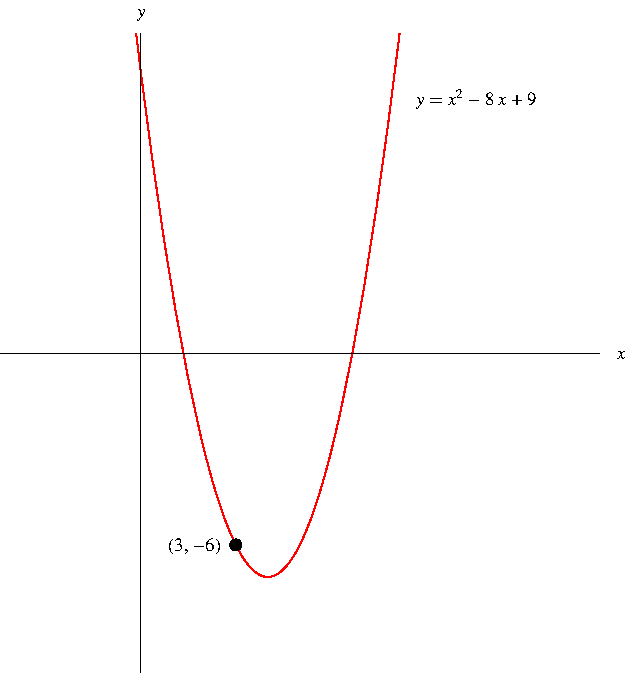
\includegraphics[height=5cm]{derivatives/pictures/03-01-ex5a.pdf}%
%}%
%\only<6->{%
%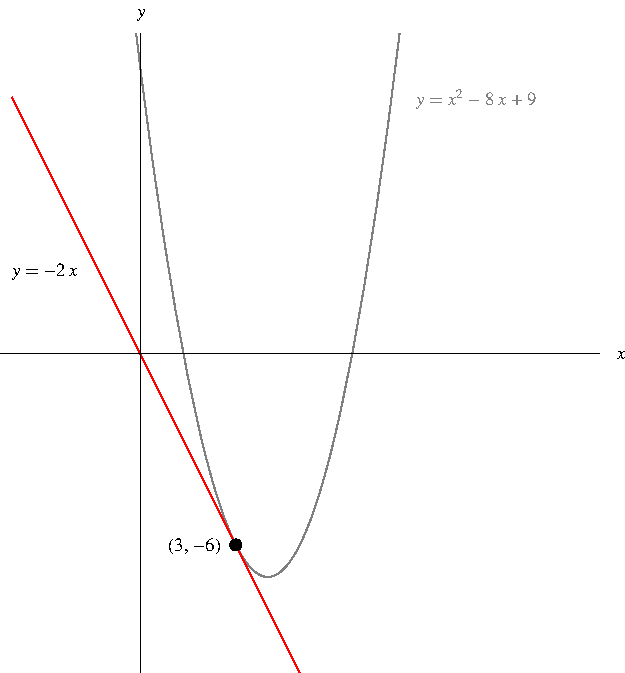
\includegraphics[height=5cm]{derivatives/pictures/03-01-ex5b.pdf}%
%}%
\column{.6\textwidth}
\begin{itemize}
\item<2->  The slope of the tangent is the derivative $f'(3)$.
\item<3->  From previous examples%Example 4, p. 138
, $f'(a) = 2a-8$.
\item<4->  Therefore $f'(3) = 2\cdot 3 - 8 = -2$.
\item<5->  Point-slope form: $y - (-6) = -2(x-3)$.
\item<6->  Slope $y$-intercept form: $y = -2x$.
\end{itemize}
\end{columns}
\end{example}
\end{frame}
% end module derivatives-ex5
